The recurrent GSN (RNN-GSN) 

\begin{equation}
	\hat{H}_t = \Phi_{h}(A^TU_{t} + b_h)
\end{equation}
\begin{equation}
	\hat{X}_t \sim GSN(X,\hat{H})
\end{equation}
\begin{equation}
	U_{t+1} = \Phi_{u}(B^TX_t + C^TU_t + b_u)
\end{equation}

where \(\Phi_h\) and \(\Phi_u\) are element-wise nonlinear functions,  $A$, $B$, $C$, $b_h$, and $b_u$ are the recurrent network parameters, and $GSN(X,\hat{H})$ is a GSN from Section \ref{gsn} trained with parameters $\Theta_1$ and $\Theta_2$.

This architecture retains separation between the recurrent part and the deep GSN part.

\begin{figure}[h!]
  \centering
    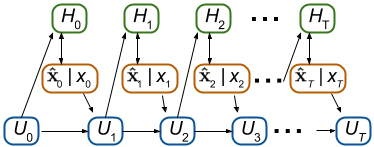
\includegraphics[width=0.45\textwidth]{rnngsn}
\caption{RNN-GSN architecture. Input distribution is X, GSN hidden layers are H, and recurrent hidden units are U.}
\end{figure}

\begin{equation}
	\hat{H}_t = \Phi_{h}(A^TU_{t} + b_h)
\end{equation}
\begin{equation}
	\hat{X}_t \sim GSN(X,H)
\end{equation}
\begin{equation}
	H_t \sim GSN(X,H)
\end{equation}
\begin{equation}
	U_{t+1} = \Phi_{u}(B^TH_t + C^TU_t + b_u)
\end{equation}

\begin{figure}[h!]
  \centering
    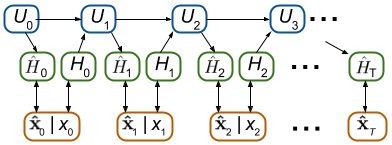
\includegraphics[width=0.45\textwidth]{rnngsn_extension}
\caption{Extension of the RNN-GSN to use both deep input-to-hidden and hidden-to-output functions with a GSN.}
\end{figure}

\subsection{Initialization strategies}
\cite{initialization}

\subsection{Algorithm}